%%%%%%%%%%%%%%%%%%%%%%%%%%%%%%%%%%%%%%%%%%%%%%%%%%%%%%%%%%%%%%%%%%%%%%%%%%%%%%%%
% Лабораторная работа 3 : Определение главных напряжений при совместном действии %                         изгиба и кручения.

% Выполнили             : Баталов Семен, Хайретдинова Диана, 2021.
%%%%%%%%%%%%%%%%%%%%%%%%%%%%%%%%%%%%%%%%%%%%%%%%%%%%%%%%%%%%%%%%%%%%%%%%%%%%%%%%

\documentclass[12pt, a4paper]{article}
\usepackage[left=2cm, right=2cm, top=2.5cm, bottom=2.5cm, nohead]{geometry}
\usepackage{graphicx}
\usepackage[utf8]{inputenc}
\usepackage[english, russian]{babel}
\usepackage{indentfirst}
\usepackage{amsmath}
\usepackage{longtable}
\usepackage{multirow}
\usepackage{array}
\usepackage{rotating}
\usepackage{subcaption}
\graphicspath{{./Figures/}}

\begin{document}
    
    \newcolumntype{M}[1]{>{\centering\arraybackslash}m{#1}}
    \renewcommand{\arraystretch}{1.3}
    
    \begin{center}
        \large{Санкт-Петербургский Государственный Университет} \\
        \large{Saint-Petersburg State University}\\
        \hfill \break
        \hfill \break
        \hfill \break
        \hfill \break
        \hfill \break
        \hfill \break
        \large{ЛАБОРАТОРИЯ ПРОЧНОСТИ МАТЕРИАЛОВ} \\
        \hfill \break
        \hfill \break
        \hfill \break
        \large{\textbf{ОТЧЕТ}} \\
        \large{\textbf{По лабораторной работе 3}} \\
        \large{<<Определение главных напряжений при совместном действии изгиба и кручения>>} \\
        \hfill \break
        \hfill \break
        \hfill \break
        \large{По дисциплине} \\
        \large{<<Лабораторный практикум, лабораторная работа>>} \\
    \end{center}
    
    \hfill \break
    \hfill \break
    \hfill \break
    \hfill \break
    \hfill \break
    \hfill \break
    
    \begin{flushright} 
        \large{Выполнили:} \\
        \hfill \break
        \large{Баталов С. А.} \\
        \large{Хайретдинова Д. Д.} \\
    \end{flushright}
    
    \hfill \break
    \hfill \break
    \hfill \break
    \hfill \break
    \hfill \break
    
    \begin{center} 
        \large{Санкт-Петербург} \\
        \large{2021} \\
    \end{center}
    
    \thispagestyle{empty}
    \newpage
    \sloppy
    
    \section{Цель работы}
    
    Напряжения на площадке, проходящей через заданную точку нагруженного тела, зависят от ее ориентации. С поворотом площадки меняются в определенной зависимости и напряжения. Совокупность напряжений, возникающих на множестве площадок, проходящих через рассматриваемую точку, называется напряженным состоянием в точке. Напряженное состояние в точке характеризуется тензором напряжений, компоненты которого представляют собой проекции векторов напряжений, действующих на трех площадках, перпендикулярных координатным осям. Диагональные компоненты тензора представляют собой нормальные составляющие напряжений, недиагональные~--~касательные.
    
    Тензор напряжений, ввиду отсутствия моментов сил, является симметричным, а это означает, что его можно диагонализовать. Оси тензора, в которых он имеет диагональный вид, называют главными осями. Соответствующие им взаимно перпендикулярные площадки называются главными площадками, а нормальные напряжения на них~--~главными напряжениями.
    
    Цель работы заключается в экспериментальном определении посредством электротензометрии положения главных осей и значений главных напряжений при плоском напряженном состоянии и сравнение результатов эксперимента с теоретическими расчетами.
    
    \newpage
    
    \section{Теоретические исследования}
    
    При кручении тонкостенного полого стержня с одновременным изгибом, в точках сечения возникают нормальное и касательное напряжения, наибольшие значения которых определяются по формулам:
    
    \begin{equation}
        \sigma_{max} = \frac{M_{x}}{W_{x}} = \frac{4Fl}{\pi d^{2} h}
        \label{eq1}
    \end{equation}
    
    \begin{equation}
        \tau_{max} = \frac{M_{k}}{W_{p}} = \frac{2Fa}{\pi d^{2} h}
        \label{eq2}
    \end{equation}
    
    Здесь $M_{x}$ и $M_{k}$~--~изгибающий и крутящий моменты в сечении, $W_{x}$ и $W_{p}$~--~моменты сопротивления сечения изгибу и кручению, $F$~--~сила, действующая на рычаг, $a$~--~длина рычага ($a = 300$~мм), $l$~--~расстояние от рычага до исследуемого сечения ($l = 260$~мм), $d$~--~средний диаметр сечения тонкостенного стержня ($d = 41$~мм), $h$~--~толщина стенки стержня ($h = 1$~мм).
    
    Главные напряжения и угол наклона $\beta$ одной из главных осей к оси стержня вычисляются по формулам:
    
    \begin{equation}
        \sigma_{1,3} = \frac{\sigma_{max}}{2} \pm \sqrt{\frac{\sigma_{max}}{2}^{2} + \tau_{max}^{2}}
        \label{eq3}
    \end{equation}
    
    \begin{equation}
        tg2\beta = \frac{2\tau}{\sigma}
        \label{eq4}
    \end{equation}
    
    Если же нам известны деформации в данной точке сечения в направлении трех осей (u, z, v), расположенных под углом $45^{\circ}$ друг к другу, то главные деформации $\varepsilon_{1}$, $\varepsilon_{3}$ и угол $\alpha$ между осью стержня и главными осями можно вычислить по формулам:
    
    \begin{equation}
        \varepsilon_{1,3} = \frac{\varepsilon_{u} + \varepsilon_{v}}{2} \pm \sqrt{\frac{1}{2} \Big[ (\varepsilon_{u} - \varepsilon_{z})^{2} + (\varepsilon_{v} - \varepsilon_{z})^{2} \Big]}
        \label{eq5}
    \end{equation}
    
    \begin{equation}
        tg2\beta = \frac{2\varepsilon_{z} - (\varepsilon_{u} + \varepsilon_{v})}{\varepsilon_{u} - \varepsilon_{v}}
        \label{eq6}
    \end{equation}
    
    \begin{equation}
        \alpha = 45^{\circ} - \beta
        \label{eq7}
    \end{equation}
    
    Значения главных напряжений в соответствии с законом Гука (связь тензора напряжений и тензора малых деформаций) будем вычислять по формулам:
    
    \begin{equation}
        \sigma_{1} = E \cdot \frac{\varepsilon_{1} + \nu \varepsilon_{3}}{1 - \nu^{2}}
        \label{eq8}
    \end{equation}
    
    \begin{equation}
        \sigma_{3} = E \cdot \frac{\varepsilon_{3} + \nu \varepsilon_{1}}{1 - \nu^{2}}
        \label{eq9}
    \end{equation}
    
    \newpage
    
    \section{Экспериментальная установка}
    
    Установка (\ref{im1}) выполнена в настольном исполнении и состоит из опорных стоек \textit{1} и \textit{2}, корпуса \textit{3}, ступенчатого вала (образца) \textit{4}, закрепленного центральным невыпадающим болтом \textit{5} рукоятки \textit{6}, рычага \textit{9} и подвески \textit{13} с гирями \textit{14}. Для снятия показаний тензорезисторов \textit{15}, наклеенных на ступень большого диаметра образца \textit{4}, измеритель деформации ИДТЦ-01 подключается к разъему \textit{16}.
    
    \begin{figure}[h]
        \centering
        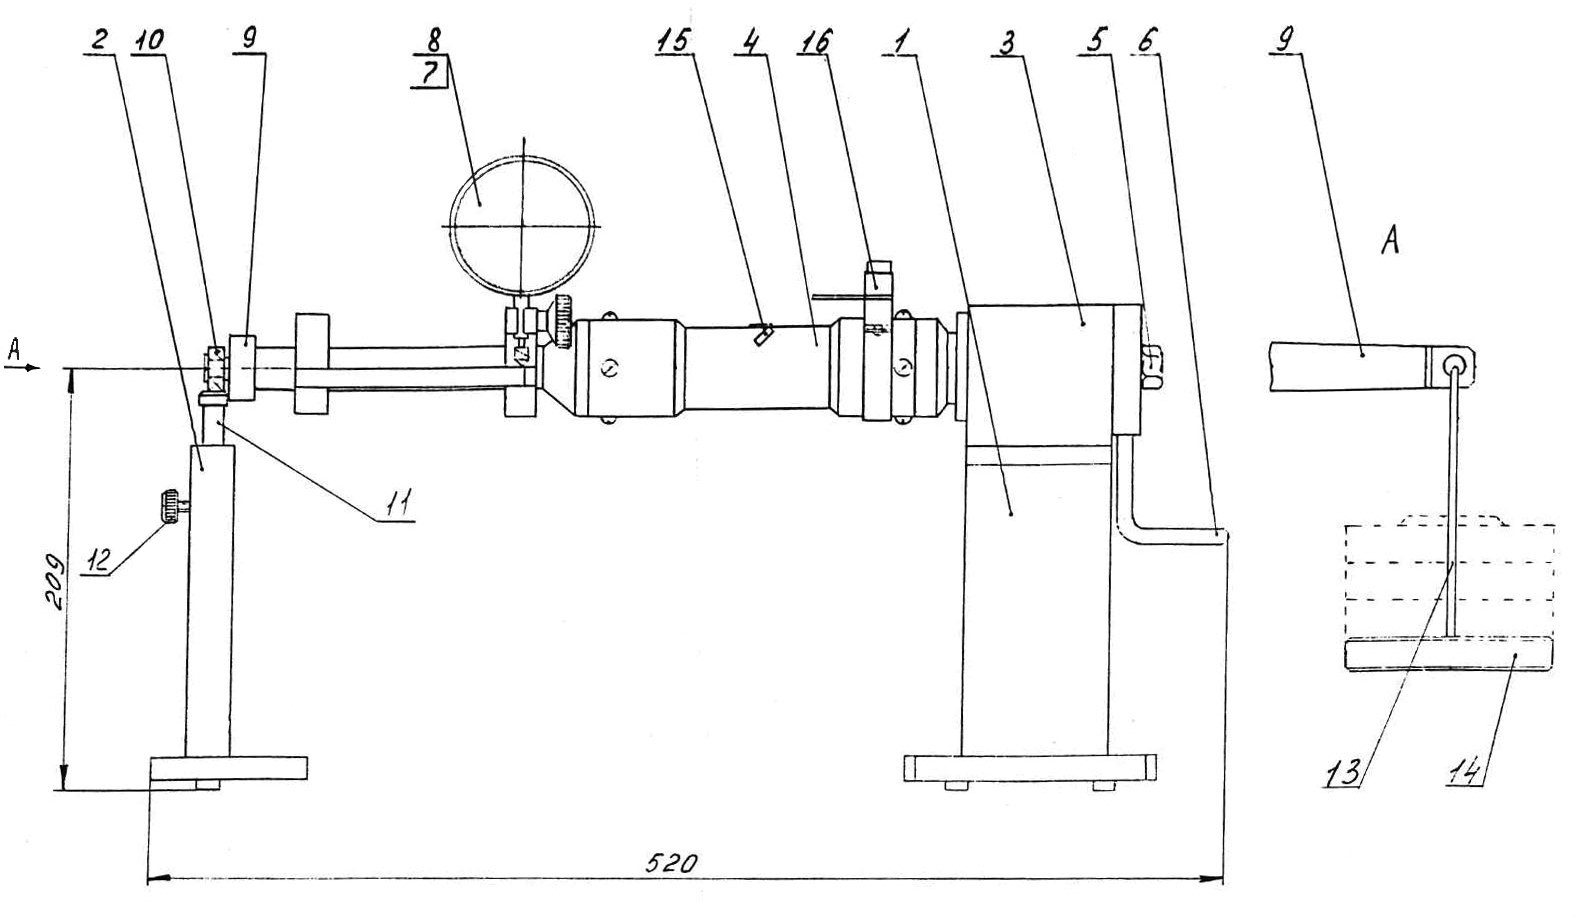
\includegraphics[width = 15cm]{image_1.jpg}
        \caption{Схема установки.}
        \label{im1}
    \end{figure}
    
    Для работы используется образец большего диаметра с наклеенными в среднем сечении тремя тензорезисторами (один вдоль оси, а два других под углом $45^{\circ}$ к ней). Для создания в сечении образца совместного кручения и изгиба необходимо опустить упор \textit{11} стойки \textit{2} так, чтобы он не касался подшипника \textit{10}. Положение упора фиксируется винтом \textit{12}.
    
    \newpage
    
    \section{Эксперимент}
    
    В данной работе при плоском напряженном состоянии проводится определение главных осей тензоров напряжений и деформаций посредством электротензометрии, также определяются соответствующие главные напряжения. Важно отметить, что все вычисления и построения производились с помощью пакета Matlab, с исходным кодом программы можно ознакомиться отдельно. Начальные данные представлены в таблице~\ref{tb1}.
    
    \begin{table}[h]
        \centering
        \begin{tabular}{| M{3cm} | M{3cm} | M{3cm} |}
            \hline
            Величина & Значение & Размерность \\
            \hline
            $a$ & 300 & \multirow{4}{*}{мм} \\
            $l$ & 260 & \\
            $d$ & 41 & \\
            $h$ & 1 & \\
            \hline
            $E$ & $0.7 \cdot 10^{5}$ & МПа \\
            $\nu$ & 0.33 & -- \\
            \hline
        \end{tabular}
        \caption{\centering Начальные данные.}
        \label{tb1}
    \end{table}
    
    Показания прибора были усреднены для 4 измерений, были рассчитаны изменеия деформаций для каждого тезодатчика по формулам:
    
    \begin{equation}
        \varepsilon_{z} = K \cdot \Delta n_{z}, \quad 					\varepsilon_{u} = K \cdot \Delta n_{u}, \quad 					\varepsilon_{v} = K \cdot \Delta n_{v}.
    \end{equation}
    
    Здесь $K = 6.4 \cdot 10^{-7}$~--~цена единицы дискретности измерителя деформаций. Погрешность измерений вычислили как сумму погрешности среднего для 4 измерений с доверительной вероятностью 90\% и систематической погрешности прибора $\Delta \varepsilon = 0.16 \cdot 10^{-5}$.
    
    Выполнили теоретический расчет главных напряжений и угла наклона $\beta$ одной из главных осей к оси стержня по формулам (\ref{eq1})~--~(\ref{eq4}) и экспериментальный расчет в соответствии с законом Гука по формулам (\ref{eq5})~--~(\ref{eq9}), рассчитали относительную погрешность измерений.
    
    \begin{table}[h]
        \centering
        \begin{tabular}{|M{3cm}|M{1.5cm}|M{1.5cm}|M{1.5cm}|M{1.5cm}|M{1.5cm}|M{1.5cm}|}
            \hline
            \multirow{2}{*}{Нагрузка} & \multicolumn{6}{c|}{Изменение деформации ТД} \\
            \cline{2-7}
            & \multicolumn{2}{c|}{1} & \multicolumn{2}{c|}{2} & \multicolumn{2}{c|}{3} \\
            \hline
            $F$ & $\Delta n_{z}$ &$\varepsilon_{z}$ & $\Delta n_{u}$ & $\varepsilon_{u}$ & $\Delta n_{v}$& $\varepsilon_{v}$ \\
            \hline
            $H$ & дел & $\cdot 10^{-5}$ & дел & $\cdot 10^{-5}$ & дел & $\cdot 10^{-5}$  \\
            \hline
            10 & 29 & 1.86 & 21 & 1.34 & -16 & -1.02 \\
            20 & 30 & 1.94 & 18 & 1.15 & -20 & -1.28 \\
            30 & 28 & 1.79 & 20 & 1.28 & -16 & -1.024 \\
            40 & 28 & 1.79 & 20 & 1.28 & -19 &-1.216 \\
            \hline
            $\Delta F  =10 \text{ Н}$ && 1.84 && 1.26 && -1.14 \\
            \hline
        \end{tabular}
        \caption{\centering Изменение деформаций в зависимости от приложенной нагрузки.}
        \label{tb2}
    \end{table}
    
    \newpage
    
    \begin{table}[h]
        \centering
        \begin{tabular}{|M{3cm}|M{2cm}|M{2cm}|M{2cm}|M{2cm}|}
            \hline
            & $\sigma_{1}$ & $\sigma_{3}$ & $tg2\beta$ & $\beta$ \\
            \cline{2-5}
            & \multicolumn{2}{c|}{МПа} & -- & $\circ$ \\
            \hline
            Теория & 2.49 & -0.52 & 1.15 & 24.54 \\
            Эксперимент & 1.19 & -1.06 & 1.48 & 27.94 \\
            Погрешность & 23\% & 36\%  & 22\% & 10\% \\
            \hline
        \end{tabular}
        \caption{\centering Экспериментальные и рассчетные данные.}
        \label{tb3}
    \end{table}
    
    \begin{table}[h]
        \centering
        \begin{tabular}{|M{1cm}|M{2cm}| M{2cm} | M{2cm} | M{2cm} |}
            \hline
            \multirow{2}{*}{№} & $F$ & $n_{z}$ & $n_{u}$ & $n_{v}$ \\
            \cline{2-5}
            & Н & \multicolumn{3}{c|}{дел} \\
            \hline
            0 & 0 & 966 & 824 & 851 \\
            \hline
            \multirow{4}{*}{1} & 10 & 995 & 847 & 835 \\
            &20 & 1026 & 865 & 816 \\
            &30 & 1053 & 885 & 800 \\
            &40 & 1082 & 904 & 780 \\
            \hline
            \multirow{4}{*}{2} & 10 & 995 & 845 & 834 \\
            &20 & 1025 & 863 & 815 \\
            &30 & 1052 & 883 & 799 \\
            &40 & 1081 & 903 & 779 \\
            \hline
            \multirow{4}{*}{3}& 10 & 994 & 843 & 835 \\
            &20 & 1024 & 862 & 815 \\
            &30 & 1053 & 883 & 798 \\
            &40 & 1080 & 902 & 781 \\
            \hline
            \multirow{4}{*}{4} & 10 & 996 & 844 & 834 \\
            &20 & 1023 & 863 & 815 \\
            &30 & 1053 & 881 & 797 \\
            &40 & 1080 & 902 & 851 \\
            \hline
        \end{tabular}
        \caption{\centering Показания ИД при 4 измерениях.}
        \label{tb11}
    \end{table}
    
    \newpage
    
    \section{Выводы}
    
    Цель данной работы заключалась в экспериментальном определении посредством электротензометрии положения главных осей и значений главных напряжений при плоском напряженном состоянии. Все поставленные задачи были выполнены, результаты эксперимента и теоретические расчеты были сведены в отдельную таблицу.
    
    В ходе работы мы ознакомились с основными принципами электротензометрии и устройством тензодатчиков. Отклонение экспериментальных результатов от теоретических происходит из-за неточности оборудования для снятия показаний с тензодатчиков.
    
\end{document}